% Options for packages loaded elsewhere
\PassOptionsToPackage{unicode}{hyperref}
\PassOptionsToPackage{hyphens}{url}
\PassOptionsToPackage{dvipsnames,svgnames*,x11names*}{xcolor}
%
\documentclass[
  ignorenonframetext,
]{beamer}
\usepackage{pgfpages}
\setbeamertemplate{caption}[numbered]
\setbeamertemplate{caption label separator}{: }
\setbeamercolor{caption name}{fg=normal text.fg}
\beamertemplatenavigationsymbolsempty
% Prevent slide breaks in the middle of a paragraph
\widowpenalties 1 10000
\raggedbottom
\setbeamertemplate{part page}{
  \centering
  \begin{beamercolorbox}[sep=16pt,center]{part title}
    \usebeamerfont{part title}\insertpart\par
  \end{beamercolorbox}
}
\setbeamertemplate{section page}{
  \centering
  \begin{beamercolorbox}[sep=12pt,center]{part title}
    \usebeamerfont{section title}\insertsection\par
  \end{beamercolorbox}
}
\setbeamertemplate{subsection page}{
  \centering
  \begin{beamercolorbox}[sep=8pt,center]{part title}
    \usebeamerfont{subsection title}\insertsubsection\par
  \end{beamercolorbox}
}
\AtBeginPart{
  \frame{\partpage}
}
\AtBeginSection{
  \ifbibliography
  \else
    \frame{\sectionpage}
  \fi
}
\AtBeginSubsection{
  \frame{\subsectionpage}
}
\usepackage{lmodern}
\usepackage{amssymb,amsmath}
\usepackage{ifxetex,ifluatex}
\ifnum 0\ifxetex 1\fi\ifluatex 1\fi=0 % if pdftex
  \usepackage[T1]{fontenc}
  \usepackage[utf8]{inputenc}
  \usepackage{textcomp} % provide euro and other symbols
\else % if luatex or xetex
  \usepackage{unicode-math}
  \defaultfontfeatures{Scale=MatchLowercase}
  \defaultfontfeatures[\rmfamily]{Ligatures=TeX,Scale=1}
\fi
% Use upquote if available, for straight quotes in verbatim environments
\IfFileExists{upquote.sty}{\usepackage{upquote}}{}
\IfFileExists{microtype.sty}{% use microtype if available
  \usepackage[]{microtype}
  \UseMicrotypeSet[protrusion]{basicmath} % disable protrusion for tt fonts
}{}
\makeatletter
\@ifundefined{KOMAClassName}{% if non-KOMA class
  \IfFileExists{parskip.sty}{%
    \usepackage{parskip}
  }{% else
    \setlength{\parindent}{0pt}
    \setlength{\parskip}{6pt plus 2pt minus 1pt}}
}{% if KOMA class
  \KOMAoptions{parskip=half}}
\makeatother
\usepackage{xcolor}
\IfFileExists{xurl.sty}{\usepackage{xurl}}{} % add URL line breaks if available
\IfFileExists{bookmark.sty}{\usepackage{bookmark}}{\usepackage{hyperref}}
\hypersetup{
  pdftitle={Data Visualization With R},
  pdfauthor={Zack Treisman},
  colorlinks=true,
  linkcolor=Maroon,
  filecolor=Maroon,
  citecolor=blue,
  urlcolor=Blue,
  pdfcreator={LaTeX via pandoc}}
\urlstyle{same} % disable monospaced font for URLs
\newif\ifbibliography
\usepackage{color}
\usepackage{fancyvrb}
\newcommand{\VerbBar}{|}
\newcommand{\VERB}{\Verb[commandchars=\\\{\}]}
\DefineVerbatimEnvironment{Highlighting}{Verbatim}{commandchars=\\\{\}}
% Add ',fontsize=\small' for more characters per line
\usepackage{framed}
\definecolor{shadecolor}{RGB}{248,248,248}
\newenvironment{Shaded}{\begin{snugshade}}{\end{snugshade}}
\newcommand{\AlertTok}[1]{\textcolor[rgb]{0.94,0.16,0.16}{#1}}
\newcommand{\AnnotationTok}[1]{\textcolor[rgb]{0.56,0.35,0.01}{\textbf{\textit{#1}}}}
\newcommand{\AttributeTok}[1]{\textcolor[rgb]{0.77,0.63,0.00}{#1}}
\newcommand{\BaseNTok}[1]{\textcolor[rgb]{0.00,0.00,0.81}{#1}}
\newcommand{\BuiltInTok}[1]{#1}
\newcommand{\CharTok}[1]{\textcolor[rgb]{0.31,0.60,0.02}{#1}}
\newcommand{\CommentTok}[1]{\textcolor[rgb]{0.56,0.35,0.01}{\textit{#1}}}
\newcommand{\CommentVarTok}[1]{\textcolor[rgb]{0.56,0.35,0.01}{\textbf{\textit{#1}}}}
\newcommand{\ConstantTok}[1]{\textcolor[rgb]{0.00,0.00,0.00}{#1}}
\newcommand{\ControlFlowTok}[1]{\textcolor[rgb]{0.13,0.29,0.53}{\textbf{#1}}}
\newcommand{\DataTypeTok}[1]{\textcolor[rgb]{0.13,0.29,0.53}{#1}}
\newcommand{\DecValTok}[1]{\textcolor[rgb]{0.00,0.00,0.81}{#1}}
\newcommand{\DocumentationTok}[1]{\textcolor[rgb]{0.56,0.35,0.01}{\textbf{\textit{#1}}}}
\newcommand{\ErrorTok}[1]{\textcolor[rgb]{0.64,0.00,0.00}{\textbf{#1}}}
\newcommand{\ExtensionTok}[1]{#1}
\newcommand{\FloatTok}[1]{\textcolor[rgb]{0.00,0.00,0.81}{#1}}
\newcommand{\FunctionTok}[1]{\textcolor[rgb]{0.00,0.00,0.00}{#1}}
\newcommand{\ImportTok}[1]{#1}
\newcommand{\InformationTok}[1]{\textcolor[rgb]{0.56,0.35,0.01}{\textbf{\textit{#1}}}}
\newcommand{\KeywordTok}[1]{\textcolor[rgb]{0.13,0.29,0.53}{\textbf{#1}}}
\newcommand{\NormalTok}[1]{#1}
\newcommand{\OperatorTok}[1]{\textcolor[rgb]{0.81,0.36,0.00}{\textbf{#1}}}
\newcommand{\OtherTok}[1]{\textcolor[rgb]{0.56,0.35,0.01}{#1}}
\newcommand{\PreprocessorTok}[1]{\textcolor[rgb]{0.56,0.35,0.01}{\textit{#1}}}
\newcommand{\RegionMarkerTok}[1]{#1}
\newcommand{\SpecialCharTok}[1]{\textcolor[rgb]{0.00,0.00,0.00}{#1}}
\newcommand{\SpecialStringTok}[1]{\textcolor[rgb]{0.31,0.60,0.02}{#1}}
\newcommand{\StringTok}[1]{\textcolor[rgb]{0.31,0.60,0.02}{#1}}
\newcommand{\VariableTok}[1]{\textcolor[rgb]{0.00,0.00,0.00}{#1}}
\newcommand{\VerbatimStringTok}[1]{\textcolor[rgb]{0.31,0.60,0.02}{#1}}
\newcommand{\WarningTok}[1]{\textcolor[rgb]{0.56,0.35,0.01}{\textbf{\textit{#1}}}}
\usepackage{graphicx,grffile}
\makeatletter
\def\maxwidth{\ifdim\Gin@nat@width>\linewidth\linewidth\else\Gin@nat@width\fi}
\def\maxheight{\ifdim\Gin@nat@height>\textheight\textheight\else\Gin@nat@height\fi}
\makeatother
% Scale images if necessary, so that they will not overflow the page
% margins by default, and it is still possible to overwrite the defaults
% using explicit options in \includegraphics[width, height, ...]{}
\setkeys{Gin}{width=\maxwidth,height=\maxheight,keepaspectratio}
% Set default figure placement to htbp
\makeatletter
\def\fps@figure{htbp}
\makeatother
\setlength{\emergencystretch}{3em} % prevent overfull lines
\providecommand{\tightlist}{%
  \setlength{\itemsep}{0pt}\setlength{\parskip}{0pt}}
\setcounter{secnumdepth}{-\maxdimen} % remove section numbering

\pgfdeclareimage[width=3.5cm]{mcslogo}{../western_logo_hor_MCS_3C_pos.pdf}
\pgfdeclareimage[width=1cm]{ccbysa}{../ccbysa88x31.png}
\titlegraphic{\href{http://creativecommons.org/licenses/by-sa/4.0/}{\pgfuseimage{ccbysa}}
\hfill
\href{https://western.edu/program/mathematics/}{\pgfuseimage{mcslogo}}}
%\usecolortheme{wcu}
%\institute{Western Colorado University}
%\setbeamertemplate{navigation symbols}{}

\title{Data Visualization With R}
\author{Zack Treisman}
\date{Spring 2021}

\begin{document}
\frame{\titlepage}

\begin{frame}[fragile]{Philosophy}
\protect\hypertarget{philosophy}{}

Good visualizations are useful at every stage of the data analysis
process from exploration to publication.

R has multiple graphics systems. We will use two:

\begin{itemize}
\tightlist
\item
  Base R graphics are often intuitive, but limited.
\item
  \texttt{ggplot2} is robust and widely used. It takes some
  acclimatization.
\end{itemize}

Many older resources use \texttt{lattice} graphics, which started
dropping in popularity as \texttt{ggplot2} took over.

Be wary of inference based on purely exploratory data analysis. If you
look at your data until you find a pattern, and then test for that
pattern, the significance levels of that test are inflated.

\end{frame}

\begin{frame}[fragile]{Loading data}
\protect\hypertarget{loading-data}{}

Step 0 of visualizing your data with R is loading it.

\begin{itemize}
\tightlist
\item
  Clean your data spreadsheet:

  \begin{itemize}
  \tightlist
  \item
    Remove non-data (summaries, etc.)
  \item
    Fix typos
  \item
    Make good variable names

    \begin{itemize}
    \tightlist
    \item
      meaningful
    \item
      not too long
    \item
      no spaces - use under\_score or camelCaps instead
    \item
      don't start with a number
    \end{itemize}
  \item
    More good advice from
    \href{https://datacarpentry.org/spreadsheet-ecology-lesson/}{Data
    Carpentry}
  \end{itemize}
\item
  Save data as a \texttt{csv}.
\item
  Put it in the working directory, possibly in a \emph{data}
  subdirectory.
\item
  Read it in with \texttt{read.csv} or \texttt{read\_csv}.
\end{itemize}

\end{frame}

\begin{frame}[fragile]{Check the data loaded correctly}
\protect\hypertarget{check-the-data-loaded-correctly}{}

\begin{itemize}
\tightlist
\item
  Use \texttt{str} to check that all the variables have been coded
  correctly (factors, dates), and fix anything that needs fixing.
\item
  use \texttt{head} or \texttt{View} to see that the data look right.
\end{itemize}

\scriptsize

\begin{Shaded}
\begin{Highlighting}[]
\KeywordTok{str}\NormalTok{(ReedfrogPred); }\KeywordTok{head}\NormalTok{(ReedfrogPred) }\CommentTok{# data in emdbook}
\end{Highlighting}
\end{Shaded}

\begin{verbatim}
## 'data.frame':    48 obs. of  5 variables:
##  $ density : int  10 10 10 10 10 10 10 10 10 10 ...
##  $ pred    : Factor w/ 2 levels "no","pred": 1 1 1 1 1 1 1 1 2 2 ...
##  $ size    : Factor w/ 2 levels "small","big": 2 2 2 2 1 1 1 1 2 2 ...
##  $ surv    : num  9 10 7 10 9 9 10 9 4 9 ...
##  $ propsurv: num  0.9 1 0.7 1 0.9 0.9 1 0.9 0.4 0.9 ...
\end{verbatim}

\begin{verbatim}
##   density pred  size surv propsurv
## 1      10   no   big    9      0.9
## 2      10   no   big   10      1.0
## 3      10   no   big    7      0.7
## 4      10   no   big   10      1.0
## 5      10   no small    9      0.9
## 6      10   no small    9      0.9
\end{verbatim}

\end{frame}

\begin{frame}[fragile]{Exploration}
\protect\hypertarget{exploration}{}

Data are in R, now what?

\begin{itemize}
\tightlist
\item
  Check numerical summaries.
\end{itemize}

\scriptsize

\begin{Shaded}
\begin{Highlighting}[]
\KeywordTok{summary}\NormalTok{(ReedfrogPred) }\CommentTok{# data in emdbook}
\end{Highlighting}
\end{Shaded}

\begin{verbatim}
##     density        pred       size         surv          propsurv     
##  Min.   :10.00   no  :24   small:24   Min.   : 4.00   Min.   :0.1143  
##  1st Qu.:10.00   pred:24   big  :24   1st Qu.: 9.00   1st Qu.:0.4964  
##  Median :25.00                        Median :12.50   Median :0.8857  
##  Mean   :23.33                        Mean   :16.31   Mean   :0.7216  
##  3rd Qu.:35.00                        3rd Qu.:23.00   3rd Qu.:0.9200  
##  Max.   :35.00                        Max.   :35.00   Max.   :1.0000
\end{verbatim}

\normalsize

\begin{itemize}
\tightlist
\item
  Make some graphics!

  \begin{itemize}
  \tightlist
  \item
    Are there patterns that you expected to see?
  \item
    Or didn't expect to see?
  \item
    Are there problems with the data?
  \end{itemize}
\end{itemize}

\end{frame}

\begin{frame}[fragile]{Standard routines - one variable}
\protect\hypertarget{standard-routines---one-variable}{}

Graphing the distribution of a single variable means representing how
often it takes each possible value.

\begin{itemize}
\tightlist
\item
  Barplots for categorical variables. Same information as a table.
\item
  Histograms for numeric variables. Can add a density estimate.
\end{itemize}

\scriptsize

\begin{Shaded}
\begin{Highlighting}[]
\KeywordTok{par}\NormalTok{(}\DataTypeTok{mfrow=}\KeywordTok{c}\NormalTok{(}\DecValTok{1}\NormalTok{,}\DecValTok{2}\NormalTok{)) }\CommentTok{# show multiple base R plots at once}
\KeywordTok{barplot}\NormalTok{(}\KeywordTok{table}\NormalTok{(ReedfrogPred}\OperatorTok{$}\NormalTok{pred))}
\KeywordTok{hist}\NormalTok{(ReedfrogPred}\OperatorTok{$}\NormalTok{propsurv,}\DataTypeTok{freq=}\NormalTok{F); }\KeywordTok{lines}\NormalTok{(}\KeywordTok{density}\NormalTok{(ReedfrogPred}\OperatorTok{$}\NormalTok{propsurv))}
\end{Highlighting}
\end{Shaded}

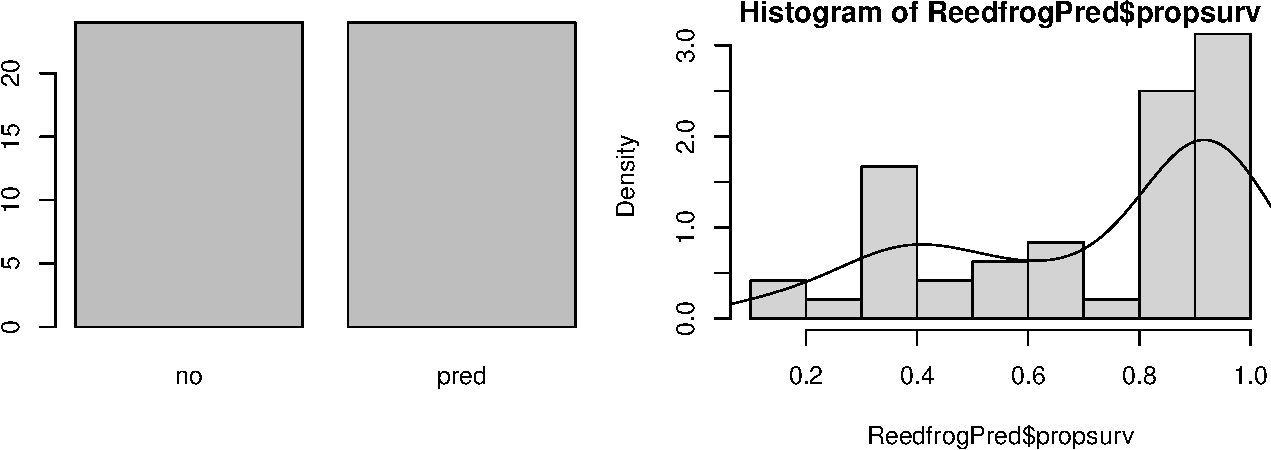
\includegraphics{data_viz_files/figure-beamer/unnamed-chunk-4-1.pdf}

\end{frame}

\begin{frame}[fragile]{Standard routines - two numeric variables}
\protect\hypertarget{standard-routines---two-numeric-variables}{}

Scatterplots show codistribution.

\begin{itemize}
\tightlist
\item
  Put the response variable on the \(y\) axis.
\end{itemize}

\scriptsize

\begin{Shaded}
\begin{Highlighting}[]
\NormalTok{p <-}\StringTok{ }\KeywordTok{ggplot}\NormalTok{(Lily_sum, }\KeywordTok{aes}\NormalTok{(vegetative, flowers)) }\OperatorTok{+}\StringTok{ }\CommentTok{# data are in emdbook}
\StringTok{  }\KeywordTok{geom_point}\NormalTok{()}
\NormalTok{p}
\end{Highlighting}
\end{Shaded}

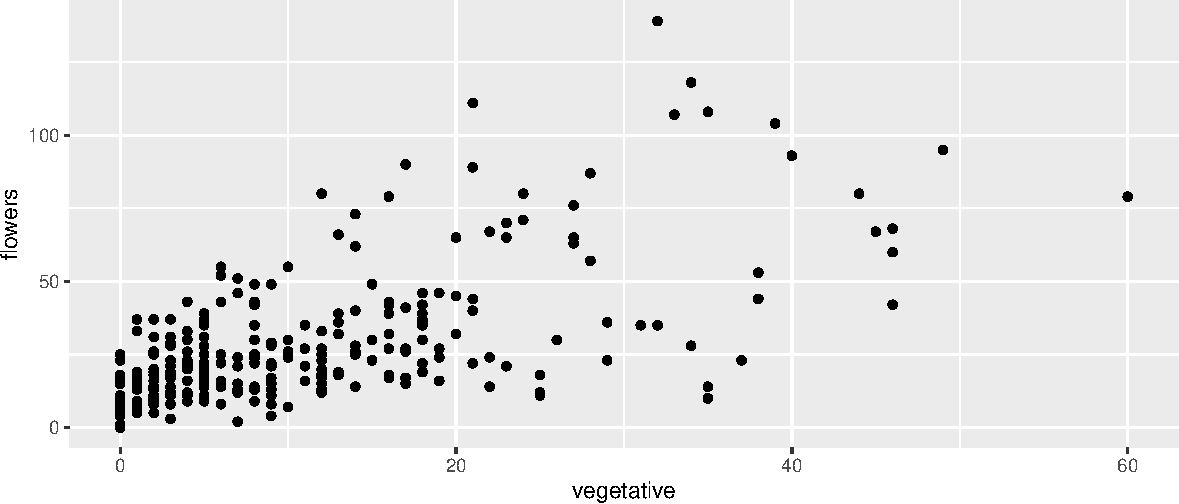
\includegraphics{data_viz_files/figure-beamer/unnamed-chunk-5-1.pdf}

\end{frame}

\begin{frame}[fragile]{Log scales}
\protect\hypertarget{log-scales}{}

Sometimes the data look better with axes on log scales.

\begin{itemize}
\tightlist
\item
  Counts
\item
  Dimesnional data
\end{itemize}

Recall log(0) is undefined so 0 values will produce warnings or errors.

\scriptsize

\begin{Shaded}
\begin{Highlighting}[]
\NormalTok{p }\OperatorTok{+}\StringTok{ }\KeywordTok{scale_x_log10}\NormalTok{() }\OperatorTok{+}\StringTok{ }
\StringTok{  }\KeywordTok{scale_y_log10}\NormalTok{()}
\end{Highlighting}
\end{Shaded}

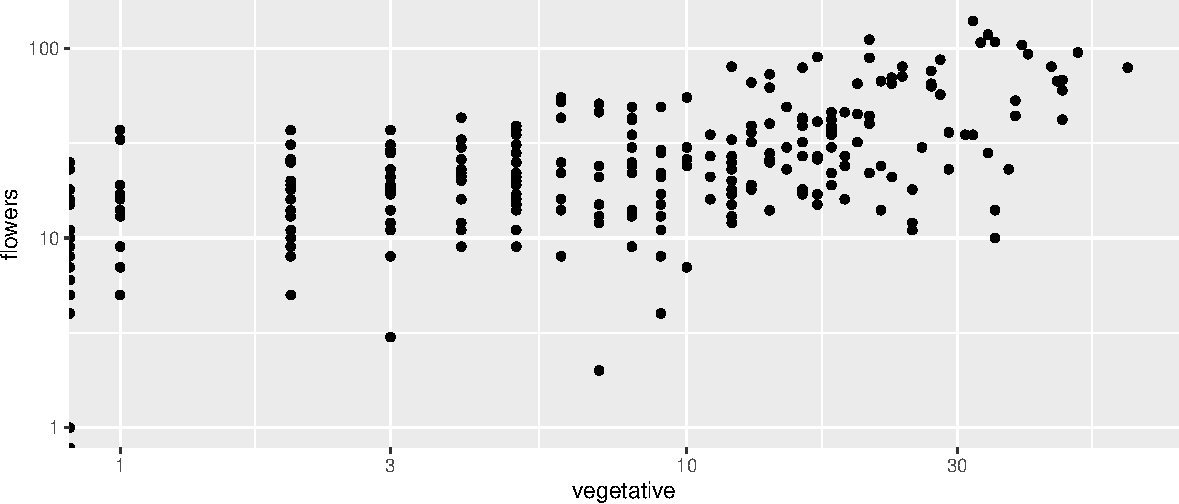
\includegraphics{data_viz_files/figure-beamer/unnamed-chunk-6-1.pdf}

\end{frame}

\begin{frame}[fragile]{Additional aesthetics}
\protect\hypertarget{additional-aesthetics}{}

Map additional variables to color, size or shape (plotting symbol).

\begin{itemize}
\tightlist
\item
  Shape can only be a categorical variable.
\item
  Size can only be a numerical variable.
\end{itemize}

Can also superimpose trendlines or other model graphs.

\scriptsize

\begin{Shaded}
\begin{Highlighting}[]
\KeywordTok{ggplot}\NormalTok{(Lily_sum, }\KeywordTok{aes}\NormalTok{(vegetative, flowers, }\DataTypeTok{color =}\NormalTok{ moisture)) }\OperatorTok{+}\StringTok{ }
\StringTok{  }\KeywordTok{geom_point}\NormalTok{() }\OperatorTok{+}
\StringTok{  }\KeywordTok{geom_smooth}\NormalTok{()}
\end{Highlighting}
\end{Shaded}

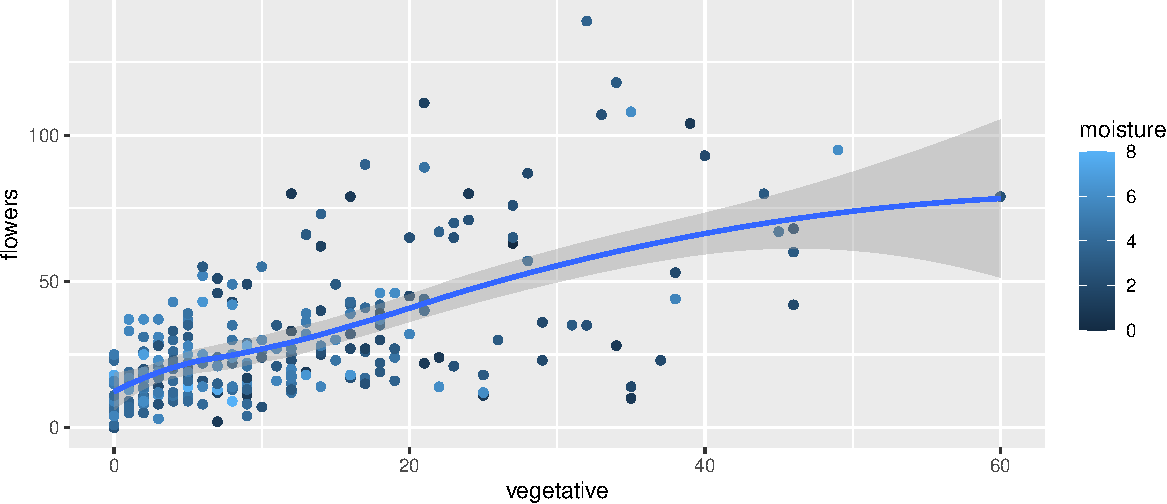
\includegraphics{data_viz_files/figure-beamer/unnamed-chunk-7-1.pdf}

\end{frame}

\begin{frame}[fragile]{Faceted plots}
\protect\hypertarget{faceted-plots}{}

Categorical variables can also be represented by making multiple plots.
Add facets to a \texttt{ggplot} and specify the variable or variables
with \texttt{facet\_wrap(\textasciitilde{}varA)} or
\texttt{facet\_grid(varB\textasciitilde{}varA)}.

\scriptsize

\begin{Shaded}
\begin{Highlighting}[]
\KeywordTok{ggplot}\NormalTok{(SeedPred, }\KeywordTok{aes}\NormalTok{(tint, taken))}\OperatorTok{+}\StringTok{ }\CommentTok{# data in emdbook}
\StringTok{  }\KeywordTok{geom_point}\NormalTok{()}\OperatorTok{+}
\StringTok{  }\KeywordTok{facet_wrap}\NormalTok{(}\OperatorTok{~}\NormalTok{species)}
\end{Highlighting}
\end{Shaded}

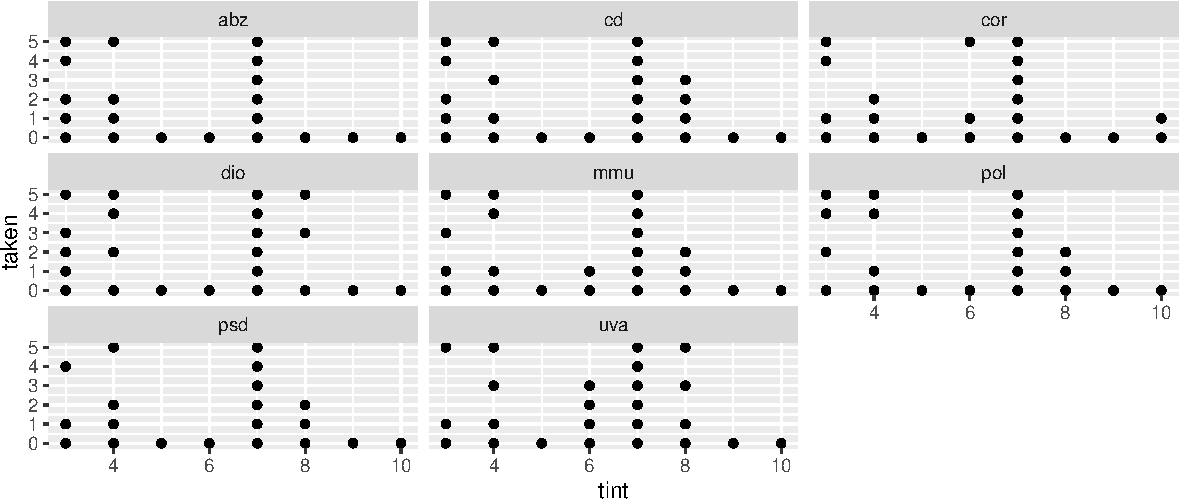
\includegraphics{data_viz_files/figure-beamer/unnamed-chunk-8-1.pdf}

\end{frame}

\begin{frame}[fragile]{Jittering and transparency}
\protect\hypertarget{jittering-and-transparency}{}

If there are many data points that take the same values, adding a jitter
to the points' position and some transparency can make patterns easier
to see.

\scriptsize

\begin{Shaded}
\begin{Highlighting}[]
\KeywordTok{ggplot}\NormalTok{(SeedPred, }\KeywordTok{aes}\NormalTok{(date, seeds))}\OperatorTok{+}\StringTok{  }\CommentTok{# data in emdbook}
\StringTok{  }\KeywordTok{geom_jitter}\NormalTok{(}\DataTypeTok{alpha=} \FloatTok{0.3}\NormalTok{)}
\end{Highlighting}
\end{Shaded}

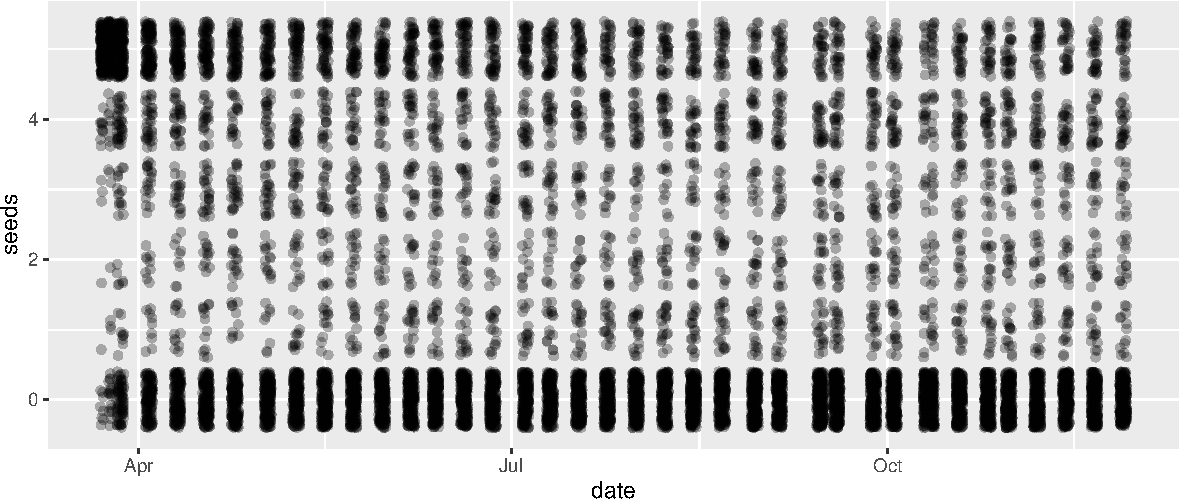
\includegraphics{data_viz_files/figure-beamer/unnamed-chunk-9-1.pdf}

\end{frame}

\begin{frame}[fragile]{Standard routines - numeric and categorical}
\protect\hypertarget{standard-routines---numeric-and-categorical}{}

If the response is numeric and all predictors are categorical, you have
some options.

\scriptsize

\begin{Shaded}
\begin{Highlighting}[]
\NormalTok{g0 <-}\StringTok{ }\KeywordTok{ggplot}\NormalTok{(OrchardSprays,}\KeywordTok{aes}\NormalTok{(}\DataTypeTok{x=}\NormalTok{treatment,}\DataTypeTok{y=}\NormalTok{decrease))}\OperatorTok{+}\StringTok{ }\CommentTok{# data in MASS}
\StringTok{  }\KeywordTok{scale_y_log10}\NormalTok{()}
\NormalTok{g_boxplot <-}\StringTok{ }\NormalTok{g0 }\OperatorTok{+}\StringTok{ }\KeywordTok{geom_boxplot}\NormalTok{()}
\NormalTok{g_point <-}\StringTok{ }\NormalTok{g0 }\OperatorTok{+}\KeywordTok{geom_point}\NormalTok{()}
\NormalTok{g_errbar <-}\StringTok{ }\NormalTok{g0 }\OperatorTok{+}\StringTok{ }\KeywordTok{stat_summary}\NormalTok{(}\DataTypeTok{fun.data=}\NormalTok{mean_cl_normal,}\DataTypeTok{geom=}\StringTok{"pointrange"}\NormalTok{)}
\NormalTok{g_dyn <-}\StringTok{ }\NormalTok{g0 }\OperatorTok{+}\StringTok{  }\KeywordTok{stat_summary}\NormalTok{(}\DataTypeTok{fun=}\NormalTok{mean,}\DataTypeTok{geom=}\StringTok{"bar"}\NormalTok{)}\OperatorTok{+}
\StringTok{  }\KeywordTok{stat_summary}\NormalTok{(}\DataTypeTok{fun.data=}\NormalTok{mean_cl_normal,}\DataTypeTok{geom=}\StringTok{"errorbar"}\NormalTok{,}\DataTypeTok{width=}\FloatTok{0.5}\NormalTok{)}
\KeywordTok{grid.arrange}\NormalTok{(g_boxplot,g_point,g_errbar,g_dyn, }\DataTypeTok{nrow=}\DecValTok{1}\NormalTok{)}
\end{Highlighting}
\end{Shaded}

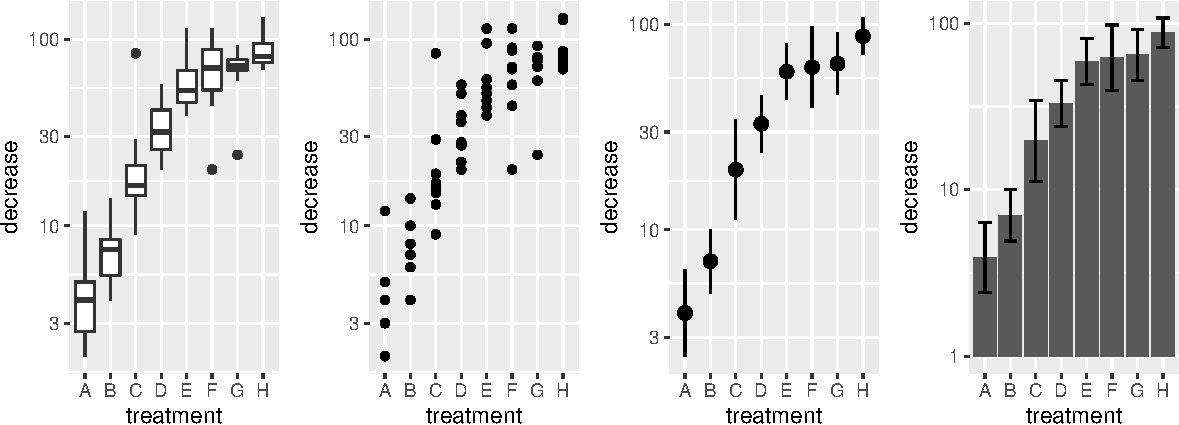
\includegraphics{data_viz_files/figure-beamer/unnamed-chunk-10-1.pdf}

\end{frame}

\begin{frame}[fragile]{Combining layers}
\protect\hypertarget{combining-layers}{}

Multiple geoms can be added to the same plot.

\scriptsize

\begin{Shaded}
\begin{Highlighting}[]
\NormalTok{g0 }\OperatorTok{+}\StringTok{ }\KeywordTok{geom_boxplot}\NormalTok{() }\OperatorTok{+}\StringTok{ }\KeywordTok{geom_point}\NormalTok{() }
\end{Highlighting}
\end{Shaded}

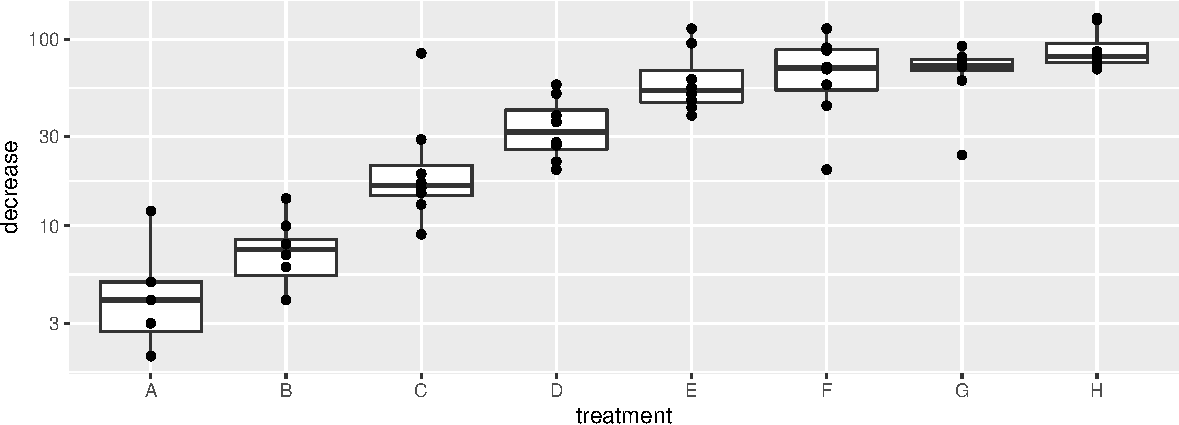
\includegraphics{data_viz_files/figure-beamer/unnamed-chunk-11-1.pdf}

\end{frame}

\begin{frame}[fragile]{Dealing with non-standard tasks}
\protect\hypertarget{dealing-with-non-standard-tasks}{}

Sometimes you need to reshape or summarize your data to plot what you
want. To produce Figure 2.1 from Bolker (2008):

\scriptsize

\begin{Shaded}
\begin{Highlighting}[]
\NormalTok{daily_avgs <-}\StringTok{ }\NormalTok{SeedPred }\OperatorTok\StringTok{   }
\StringTok{  }\KeywordTok{group_by}\NormalTok{(date, species, dist) }\OperatorTok
\StringTok{  }\KeywordTok{summarise}\NormalTok{(}\DataTypeTok{mean_seeds =} \KeywordTok{mean}\NormalTok{(seeds))}
\KeywordTok{ggplot}\NormalTok{(daily_avgs, }\KeywordTok{aes}\NormalTok{(date, mean_seeds, }\DataTypeTok{color=}\NormalTok{species, }\DataTypeTok{shape=}\NormalTok{dist)) }\OperatorTok{+}
\StringTok{  }\KeywordTok{geom_point}\NormalTok{() }\OperatorTok{+}\StringTok{ }\KeywordTok{geom_line}\NormalTok{() }\OperatorTok{+}\StringTok{ }\KeywordTok{scale_y_log10}\NormalTok{()}
\end{Highlighting}
\end{Shaded}

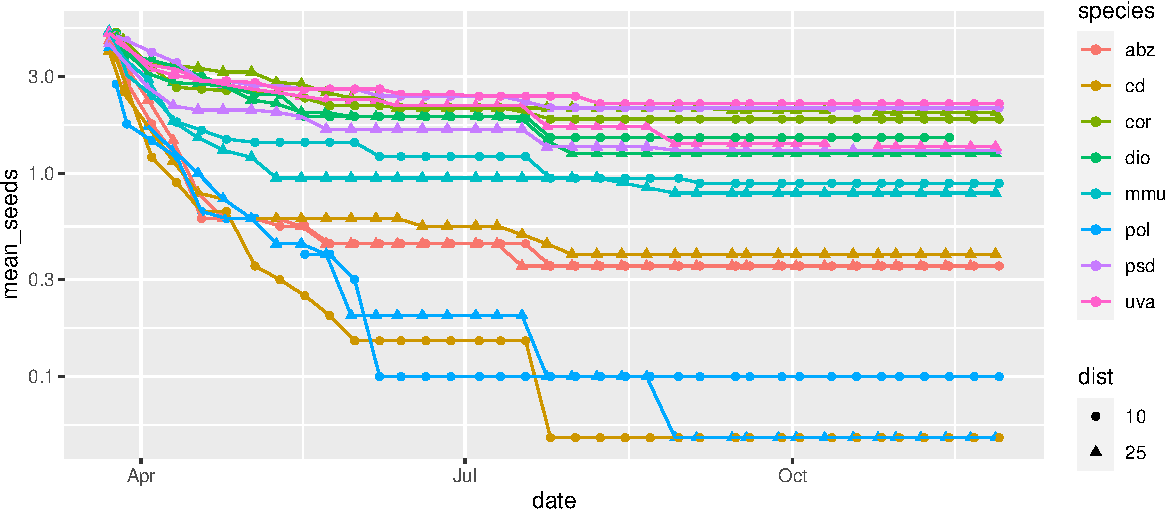
\includegraphics{data_viz_files/figure-beamer/unnamed-chunk-12-1.pdf}

\end{frame}

\begin{frame}[fragile]{Diagnostics}
\protect\hypertarget{diagnostics}{}

Assessing the validity of a model is often done graphically. \scriptsize

\begin{Shaded}
\begin{Highlighting}[]
\NormalTok{lm1 <-}\StringTok{ }\KeywordTok{lm}\NormalTok{(flowers}\OperatorTok{~}\NormalTok{vegetative, }\DataTypeTok{data =}\NormalTok{ Lily_sum)}
\KeywordTok{par}\NormalTok{(}\DataTypeTok{mfrow=}\KeywordTok{c}\NormalTok{(}\DecValTok{2}\NormalTok{, }\DecValTok{2}\NormalTok{), }\DataTypeTok{mar =} \KeywordTok{c}\NormalTok{(}\DecValTok{4}\NormalTok{, }\DecValTok{4}\NormalTok{, }\DecValTok{2}\NormalTok{, }\DecValTok{2}\NormalTok{)) }\CommentTok{# see all 4 plots at once}
\KeywordTok{plot}\NormalTok{(lm1)}
\end{Highlighting}
\end{Shaded}

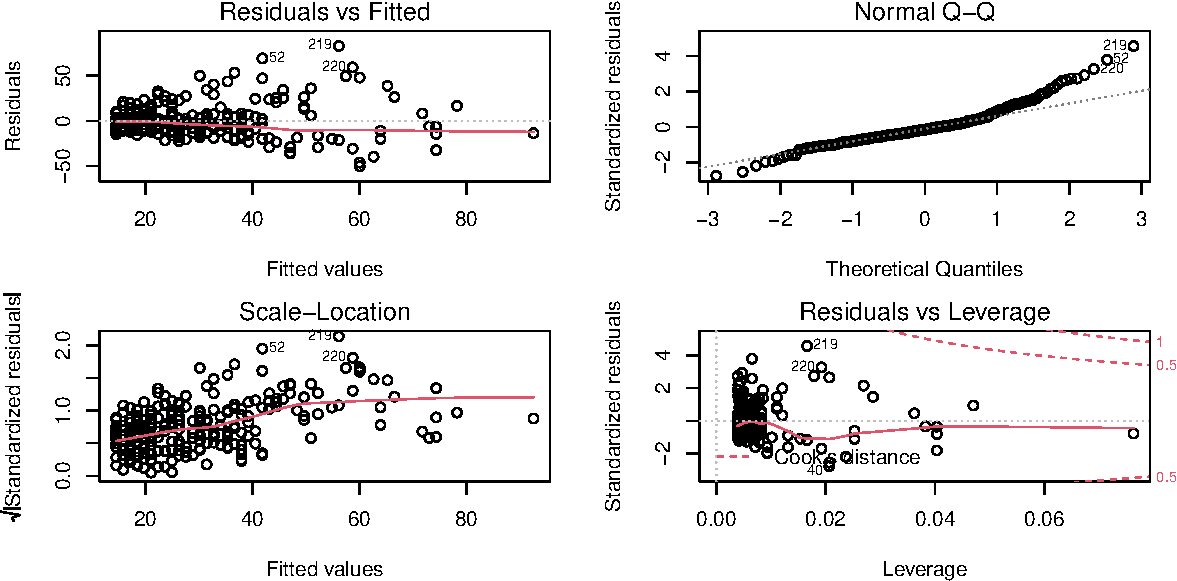
\includegraphics{data_viz_files/figure-beamer/unnamed-chunk-13-1.pdf}

\begin{Shaded}
\begin{Highlighting}[]
\KeywordTok{par}\NormalTok{(}\DataTypeTok{mfrow=}\KeywordTok{c}\NormalTok{(}\DecValTok{1}\NormalTok{, }\DecValTok{1}\NormalTok{), }\DataTypeTok{mar =} \KeywordTok{c}\NormalTok{(}\DecValTok{4}\NormalTok{, }\DecValTok{4}\NormalTok{, }\FloatTok{0.75}\NormalTok{, }\FloatTok{0.5}\NormalTok{)) }\CommentTok{# restore graphics parameters}
\end{Highlighting}
\end{Shaded}

\end{frame}

\begin{frame}[fragile]{Residuals v. predictors}
\protect\hypertarget{residuals-v.-predictors}{}

The \texttt{plot} method for \texttt{lm} doesn't show residuals against
predictors. Do that manually.

\scriptsize

\begin{Shaded}
\begin{Highlighting}[]
\KeywordTok{plot}\NormalTok{(lm1}\OperatorTok{$}\NormalTok{residuals}\OperatorTok{~}\NormalTok{Lily_sum}\OperatorTok{$}\NormalTok{vegetative)}
\KeywordTok{abline}\NormalTok{(}\DataTypeTok{h=}\DecValTok{0}\NormalTok{)}
\end{Highlighting}
\end{Shaded}

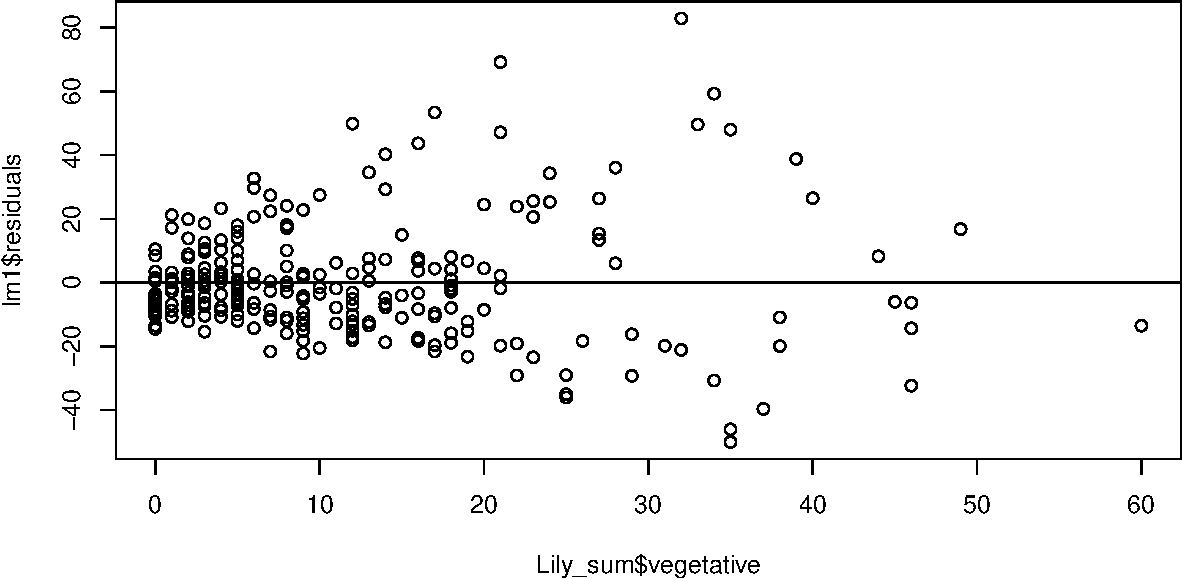
\includegraphics{data_viz_files/figure-beamer/unnamed-chunk-14-1.pdf}

\end{frame}

\begin{frame}[fragile]{Fine tune and save graphics for presentation}
\protect\hypertarget{fine-tune-and-save-graphics-for-presentation}{}

\scriptsize

\begin{Shaded}
\begin{Highlighting}[]
\NormalTok{emd2}\FloatTok{.1}\NormalTok{<-}\KeywordTok{ggplot}\NormalTok{(daily_avgs,}\KeywordTok{aes}\NormalTok{(date,mean_seeds,}\DataTypeTok{color=}\NormalTok{species,}\DataTypeTok{shape=}\NormalTok{dist))}\OperatorTok{+}
\StringTok{  }\KeywordTok{geom_point}\NormalTok{() }\OperatorTok{+}\StringTok{ }\KeywordTok{geom_line}\NormalTok{() }\OperatorTok{+}\StringTok{ }\KeywordTok{scale_y_log10}\NormalTok{() }\OperatorTok{+}
\StringTok{  }\KeywordTok{labs}\NormalTok{(}\DataTypeTok{y=}\StringTok{"Mean seeds remaining"}\NormalTok{, }\DataTypeTok{x =} \StringTok{"Date"}\NormalTok{, }
       \DataTypeTok{color =} \StringTok{"Species"}\NormalTok{, }\DataTypeTok{shape =} \StringTok{"Distance to Forest"}\NormalTok{) }\OperatorTok{+}
\StringTok{  }\KeywordTok{scale_color_brewer}\NormalTok{(}\DataTypeTok{palette =} \StringTok{"Dark2"}\NormalTok{) }\OperatorTok{+}
\StringTok{  }\KeywordTok{theme_bw}\NormalTok{()}
\NormalTok{emd2}\FloatTok{.1}
\end{Highlighting}
\end{Shaded}

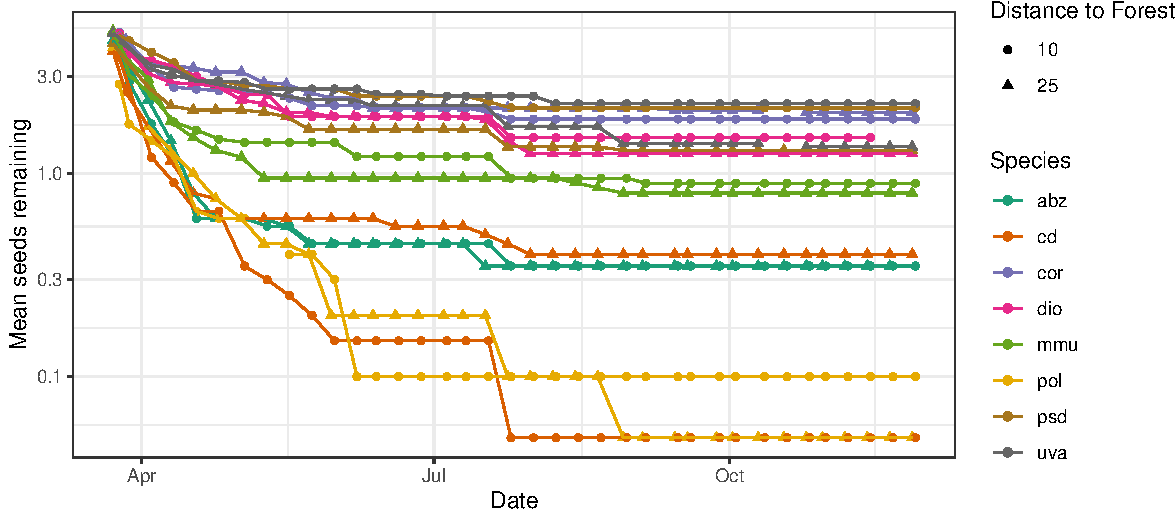
\includegraphics{data_viz_files/figure-beamer/unnamed-chunk-15-1.pdf}

\begin{Shaded}
\begin{Highlighting}[]
\KeywordTok{ggsave}\NormalTok{(}\StringTok{"figures/BolkerFig2.1.tiff"}\NormalTok{, }\DataTypeTok{plot=}\NormalTok{emd2}\FloatTok{.1}\NormalTok{, }
       \DataTypeTok{width =} \DecValTok{10}\NormalTok{, }\DataTypeTok{height =} \DecValTok{4}\NormalTok{, }\DataTypeTok{units =} \StringTok{"cm"}\NormalTok{, }\DataTypeTok{dpi =} \DecValTok{800}\NormalTok{)}
\end{Highlighting}
\end{Shaded}

\end{frame}

\begin{frame}{Opinions on graphical style}
\protect\hypertarget{opinions-on-graphical-style}{}

Plenty of people with good ideas about style.

\begin{itemize}
\tightlist
\item
  \href{https://www.springer.com/gp/book/9780387245447}{Leland
  Wilkinson}
\item
  \href{https://www.edwardtufte.com/tufte/books_vdqi}{Edward Tufte}
\item
  \href{https://www.stat.purdue.edu/~wsc/}{William Cleaveland}
\item
  \href{http://www.stat.columbia.edu/~gelman/graphics.course/p755.pdf}{Andrew
  Gelman}
\end{itemize}

Some graph types are controversial. That doesn't mean never use them,
but if you do, be aware of the criticisms.

\begin{itemize}
\tightlist
\item
  Pie charts, dynamite plots, dual-axes plots
\end{itemize}

\end{frame}

\begin{frame}{References}
\protect\hypertarget{references}{}

\hypertarget{refs}{}
\leavevmode\hypertarget{ref-bolker}{}%
Bolker, Benjamin M. 2008. \emph{Ecological Models and Data in R}.
Princeton University Press.

\end{frame}

\end{document}
